\section{Entwurf des abzubildenden Geschäftsprozesses}

Das zu implementierende System soll mittels Microservicearchitektur umgesetzt werden. Die einzelnen Services sollen das Saga-Pattern verwenden, um miteinander zu kommunizieren. Fehler in der Geschäftslogik sollen kompensiert werden. Für jeden auszuführenden Schritt soll es also einen kompensierenden Schritt geben. 

\subsection{Geschäftsprozess}

Als abzubildender Geschäftsprozess soll ein Bestell- und Liefervorgang eines Online-Shops dienen. Der Bestellvorgang soll durch das Platzierung einer Bestellung ausgelöst werden. Die Benutzeroberfläche gehört nicht zum Scope des umzusetzenden Systems. 

Als Ausgangspunkt soll folgender Geschäftsprozess dienen:

\begin{figure}[h!]
	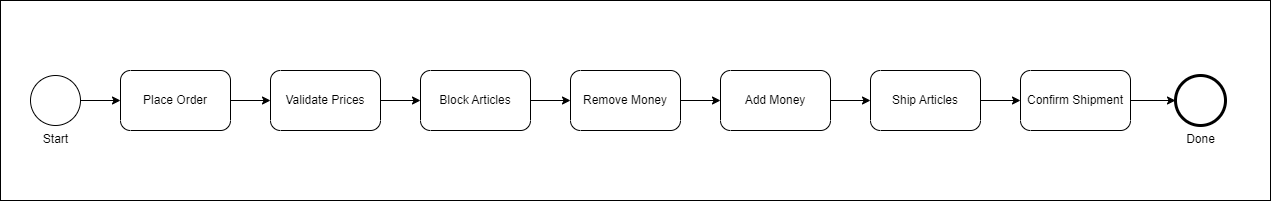
\includegraphics[width=\linewidth]{figures/SimplifiedBusinessProcess.png}
\end{figure}


% TODO Diagramm für den vereinfachten Prozess

Die zum Prozess gehörenden Schritte sind folgende:
\begin{enumerate}
	\item Entgegennehmen der Bestellung: Die Bestellung wird über ein imaginäres Frontend entgegengenommen. Dieses Frontend baut einen Request auf und sendet diesen per Http-Schnittstelle an das Backend. Dort wird der Request entgegengenommen und muss alle für die Abwicklung der Bestellung erforderlichen Daten enthalten. Dazu gehören der bestellende Nutzer, die geforderten Artikel und die Zahlungsinformationen. Beim Entgegennehmen wird die Bestellung initialisiert.
	\item Validierung des Preises: Der Bestellungsrequest enthält eine Liste von den gewünschten Produkten und dem bekannten Preis pro Produkt. Um zu überprüfen, ob der dem Nutzer (dem Frontend) bekannte Preis mit dem aktuellen Preis übereinstimmt, muss dieser validiert werden. % TODO warum ist dieser Schritt notwendig	
	\item Blockieren der Artikel: Die geforderten Artikel sollten für diese Bestellung reserviert werden, bis der Bestellvorgang abgeschlossen ist. In einem Online-Shop wird angezeigt, wieviele Artikel auf Lager vorrätig sind. Beim Blockieren der Artikel wird dieser Betrag verändert. Somit sehen andere Nutzer nach Ausführung dieses Schrittes den aktuellen Wert der vorrätigen Artikel. 
	\item Zahlungsabwicklung: Der berechnete Preis der Bestellung muss vom Konto des Kunden abgebucht und auf das Konto des Händlers gutgeschrieben werden. Die Konten des Kunden und des Online-Shop-Besitzers müssen nicht bei derselben Bank liegen. In diesem Schritt muss also eine verteilte Transaktion stattfinden.
	\item Auslösen der Lieferung: Die blockierten Artikel werden versendet. Dieser Prozess dauert einen längeren Zeitraum an.
	\item Abschluss der Lieferung: Die Saga ist abgeschlossen.
\end{enumerate}

\subsection{Services}
Aus der Beschreibung des Geschäftsprozesses lassen sich folgende Services ableiten:

\begin{tabular}[h]{|l|l|}
	\hline
	Name des Services & Aufgabe \\ \hline
	Frontend & GUI, Anzeige der Produkte, Aufnahme der Bestellung, Platzieren der Bestellung \\ \hline
	OrderService & Entgegennehmen der Bestellung, Koordinierung des Bestellprozesses \\ \hline
	ArticleService & API für die angebotenen Produkte und Preise \\ \hline
	StockService & Informationen über Lagerstand, Auslösen des Lieferprozesses \\ \hline
	BankingServices & Schnittstellen für das Erhöhen und Verringern von Geldbeträten eines Kontos \\ \hline
\end{tabular}

\subsection{Transaktionen}
Sieht man den gesamten Geschäftsprozess als Transaktion, wären folgende lokale Transaktionen Teil der globalen Transaktion, die durch das Platzieren der Bestellung ausgelöst werden:
\begin{enumerate}
	\item $T_1$: OrderService - Initialisieren der Bestellung
	\item $T_2$: OrderService, ArticleService - Abfragen und Validieren des Preises für jeden geforderten Artikel 
	\item $T_3$: StockService - Blockieren der Artikel
	\item $T_4$: BankingService des Kundenkontos - Verringern des Geldbetrages des Kundenkontos
	\item $T_5$: BankingService des Händlerkontos - Erhöhen des Geldbetrages des Händlerkontos
	\item $T_6$: StockService - Lieferung auslösen
	\item $T_7$: StockService - Lieferung bestätigen
\end{enumerate}

Nach der Funktionsweise des Saga-Patterns muss für jede lokale Transaktion eine Kompensierung angeboten werden:

\begin{tabular}[h]{|l|l|}
	\hline
	Transaktion & Kompensierung \\ \hline
	$T_1$ & - \\ \hline
	$T_2$ & - \\ \hline
	$T_3$ & $C_3$: StockService - Freigeben der Artikel \\ \hline
	$T_4$ & $C_4$: Erhöhen des Geldbetrages des Kundenkontos \\ \hline
	$T_5$ & $C_5$: Verringern des Geldbetrages des Händlerkontos \\ \hline
	$T_6$ &  - \\ \hline
	$T_7$ &  - \\ \hline
\end{tabular}


\section{Spezifikation der Services}

Für die Realisierung des Microservicesystems im Rahmen dieser Arbeit wurde die Orchestrierung gewählt. % TODO Begründung warum
Die Rolle des Koordinators übernimmt der OrderService. Der OrderService übernimmt die Annahme des Bestellprozesses und löst somit die Saga aus. 

\subsection{Frontend}
\subsubsection{Funktionalitäten}
In einem Online-Shop interagiert der Kunde per Frontend mit der Anwendung. Das Frontend soll übernimmt die grafische Schnittstelle zwischen Backend und dem Nutzer. Dazu gehört vor Allem die Darstellung der Artikel in einer Katalogansicht. Die darzustellenden Daten für eine solche Liste müssen zumindest Artikelbezeichnung und Artikelpreis enthalten. Diese Daten sollten aus einer API für Artikeldaten stammen. Darüber hinaus muss das Frontend einen Prozess unterstützen, in dem der Kunde ein Formular ausfüllt, welches die erforderlichen Daten für das Platzieren einer Bestellung enthält. Dazu gehört ein Warenkorbsystem sowie eine Authorisierung und Authentifizierung der Zahlungsidentität des Kunden. Die Bestellung kann also als Objekt mit folgenden Feldern zusammengefasst werden:
\begin{itemize}
	\item Consument
	\begin{itemize}
		\item BankId
		\item UserId
	\end{itemize}
	\item Liste der zu bestellenden Artikel
	\begin{itemize}
		\item ArticleId
		\item ArticlePrices
		\item Amount
	\end{itemize}
\end{itemize}

Dieses Objekt kann an das Backend gesendet werden.

\subsection{ArticleService}
\subsubsection{Funktionalitäten}
Dieser Service ist ein Service zum reinen Lesen der Produktdaten. Er soll eine Schnittstelle zur Verfügung stellen, die dem Frontend ermöglicht, den Produktkatalog abzufragen und darzustellen. Das Backend muss außerdem die Möglichkeit haben, die im Request enthaltenen Artikelpreise zu validieren. Dazu benötigt der Service eine Produktdatenbank. Da dieser Service ausschließlich die Produktdaten als Ressource behandelt, kann er RESTful implementiert werden.

\subsubsection{Endpunkte}
Diese Schnittstelle liefert eine Liste von Produkten. 

$GET \ /products$

Diese Schnittstelle liefert für eine ProduktId das zugehörige Produkt.

$GET \ /products/{productId}$

\subsubsection{Datenbanktabellen}
Die Produktdatenbank benötigt lediglich eine Tabelle mit den Artikeldaten.
% TODO ER-Diagramm oder create statement

\subsubsection{Kompensierung}
Da dieser Service den Systemzustand nicht verändert, sondern lediglich lesend auf die Produktdaten zugreift, gibt es keine kompensierenden Endpunkte.

\subsection{StockService}
\subsubsection{Funktionalitäten}
Dieser Service soll dazu dienen, den Lagerbestand der vorhandenen Artikel zu verwalten. Dazu gehört die Reservierung von Artikeln, das Auslösen und der Abschluss einer Lieferung. 
\paragraph{Darstellung des aktuellen Lagerbestands}
Um dies zu erlauben, muss der aktuelle Lagerstand in einer Tabelle hinterlegt sein. Die Tabelle muss den aktuell verfügbaren Bestand pro Artikel ausdrücken. 
\paragraph{Reservierung von Artikeln}
Um eine Reservierung zu ermöglichen, muss es eine weitere Tabelle geben, die eine Menge von blockierten Artikeln für einen bestimmten Bestellprozess blockiert. Beim Reservieren verringert sich der Bestand in der Bestandstabelle und erhöht sich in der Reservierungstabelle. Um die Konsistenz zu gewährleisten, müssen beide Operationen in einer lokalen Transaktion ausgeführt werden. Die Summe der vorrätigen Artikel und der reservierten Artikel darf sich nicht verändern bis der Artikel geliefert wird und somit tatsächlich nicht mehr vorrätig ist.
\paragraph{Auslösen einer Lieferung}
Um das Auslösen und Abschließen einer Lieferung zu ermöglichen, muss es eine Tabelle geben, die den Inhalt einer Lieferung und einen Status enthält.
Wenn eine Lieferung ausgelöst wird, werden die für diesen Vorgang reservierten Artikel aus der Reservierungstabelle entfernt und in der Lieferungstabelle eingefügt. Um Konsistenz zu gewährleisten, muss dies in einer lokalen Transaktion erfolgen. 

\subsubsection{Endpunkte}
Die Schnittstelle zum Reservieren von Produkten empfängt einen Http-Body mit folgenden Daten:
\begin{itemize}
	\item Vorgangsnummer
	\item Liste von Produkten
	\begin{itemize}
		\item ArtikelId
		\item Anzahl
	\end{itemize}
\end{itemize}

$POST \ /blocked-articles$

Die Schnittstelle zum Auslösen einer Bestellung muss lediglich die Vorgangsnummer enthalten. 

$GET \ /shipments/{shipmentId}$

\subsubsection{Datenbanktabellen}
articlestock, blockedarticles, shipments

\subsubsection{Kompensierung}
Die Blockierung eines Artikels muss kompensiert werden können, da sonst der blockierte Artikel nach Abbruch einer Bestellung nicht wieder freigegeben würde. Deshalt muss diese Kompensierung die Einträge aus der Blockierungstabelle entfernen und die Anzahl auf den Lagerbestand addiert werden. Dies soll ebenfalls in einer lokalen Transaktion ablaufen, um Konsistenz zu wahren.

Das Auslösen einer Lieferung ist nicht in dem Sinne kompensierbar. Das liegt nicht an dem System, sondern am repräsentierten Geschäftsprozess. Eine Stornierung ist im Rahmen dieser Umsetzung nicht vorgesehen. 

\subsection{BankingServices}
\subsubsection{Funktionalitäten}
Im Geschäftsprozess wurde definiert, dass die Transaktion das Geldbetrag des Kundenkontos und des Händlerkontos in zwei separaten Transaktionen abwickeln können soll. Somit muss der BankingService jeweils eine Transaktion zum Erhöhen und zum Verringern des Geldbetrages anbieten. Der BankingService soll am Ende in zwei Instanzen laufen, die zwei verschiedene Banken darstellen sollen. Kunden- und Käuferkonto können, müssen aber nicht bei derselben Bank liegen. 

Um dies zu ermöglichen benötigt der BankingService eine Tabelle, die seine Nutzer enthält. Zusätzlich benötigt der Service eine Tabelle, die den aktuellen Geldbetrag jedes Nutzers enthält. Außerdem sollten die einzelnen Transaktionen jedes Nutzers in einer separaten Tabelle gesichert werden. Für die reine Implementierung dieser Anwendung wäre dies nicht notwendig. Für den Nutzer eines BankingServices ist neben dem Kontostand auch die Liste an getätigten Transaktionen interessant, um die Ausgaben und Einnahmen zuordnen zu können. Im Rahmen dieser Implementierung wird die Tabelle zusätzlich für Analysezwecke verwentet werden.
 
Bei einer Anfrage, den Geldbetrag eines konkreten Nutzers zu erhöhen, wird in einer lokalen Transaktion der Betrag des Kontos in der UserCredit-Tabelle erhöht und die Differenz in der Transaktion-Tabelle eingetragen. 

Der Service darf Anfragen zum Geld verringern ablehnen, wenn die Verringerung den Kontostand in den negativen Bereich fallen lassen würde. In diesem Fall wird die Transaktion abgebrochen. %TODO usertransactiontabelle
 
\subsubsection{Endpunkte}
$POST \ /add-money$

$POST \ /remove-money$

\subsubsection{Datenbanktabellen}
user, usercredit, usertransaction

\subsubsection{Kompensierung}
Beide angebotenen Operationen benötigen eine zugehörige Kompensation, da sie den Datenbestand verändern. Die Verwendung des jeweils anderen Endpunktes ist semantisch bereits korrekt. Der Klarheit halber sollen zwei weitere Entpunkte eingeführt werden, die nur für die Kompensation verwendet werden sollen.

$POST \ /add-money-compensation$

$POST \ /remove-money-compensation$

\section{OrderService}
\subsubsection{Funktionalitäten}
Der OrderService übernimmt die Rolle des Koordinators im Orchestrator-Saga-Patterns. Die Bestellung wird entgegengenommen und vom OrderService initialisiert. Zur Initialisierung gehört die Generierung einer Vorgangsnummer sowie das Abspeichern der Bestellung in einer separaten Tabelle. Anhand dieser Tabelle wird persistiert, an welcher Stelle der Ausführung die Saga sich befindet, und in welchem Status die Bestellung ist. Die etwaigen ausgeführten Kompensationsschritte sind in ihrer eigenen Tabelle und werden der Vorgansnummer zugeordnet. Die gewünschten Artikel einer Bestellung sind in eine separate Tabelle ausgelagert und verweisen auf die Saga-Tabelle. 

Als Koordinator hat dieser Service die Verantwortung, die an der Saga beteiligten Services korrekt aufzurufen. Die Reihenfolge und die getroffenen Entscheidungen repräsentieren die Geschäftslogik. 

Nach jedem Schritt persistiert der OrderService den Erfolg oder Misserfolg. Außerdem ruft der Service nach Feststellung eines Misserfolgs die Kompensierungskette auf. 

\subsubsection{Endpunkte}
$POST \ /order$

\subsubsection{Datenbanktabellen}

ordersaga, requestedarticle, ordersagacompensations

\subsubsection{Durchlauf einer erfolgreichen Saga}
% TODO Ablaufdiagramm mit nummerierten Pfeilen

\subsubsection{Durchlauf einer gescheiterten, kompensierten Saga}
% TODO Ablaufdiagramm mit nummerierten Pfeilen

\subsubsection{Durchlauf einer gescheiterten, nichtkompensierten Saga}
% TODO Ablaufdiagramm mit nummerierten Pfeilen